This chapter will discuss the process of implementing the application. The justification of the technologies used along with the benefits, and, challenges they potentially presented will be discussed here. A comparative study \cite{compStudy} was performed in the early stages to help decide what technologies were best suited to the task.

\section{Version Control}
Version control is required to have been used throughout the duration of the project. Version control allows us to keep track and manage changes made to source code and other software artefacts. Good utilization of version control is critical to the success of a project, and helps to keep a project organised.
\subsection{GitHub \& Git}
GitHub \cite{github} is a platform widely used throughout the industry to store software projects online. GitHub allows users to create Git repositories \cite{git} that contain the files used within a project along with their version history. This combination is widely used within the industry due to the distributed version control and the various tools offered by GitHub to enhance the developer experience. Both these tools were very familiar so made this a simple choice. 
\subsubsection{Feature Branching}
An advantage of using a distributed version control system such as Git is how easy branching is due to the developer being able to create multiple branches at a local level. Feature branching was used throughout this project (see \ref{fig:branching}), with new features being developed in local feature branches and then merged back with the main branch upon completion.  
\begin{figure}[!htbp]
    \centering
    \begin{subfigure}[b]{0.90\textwidth}
        \frame{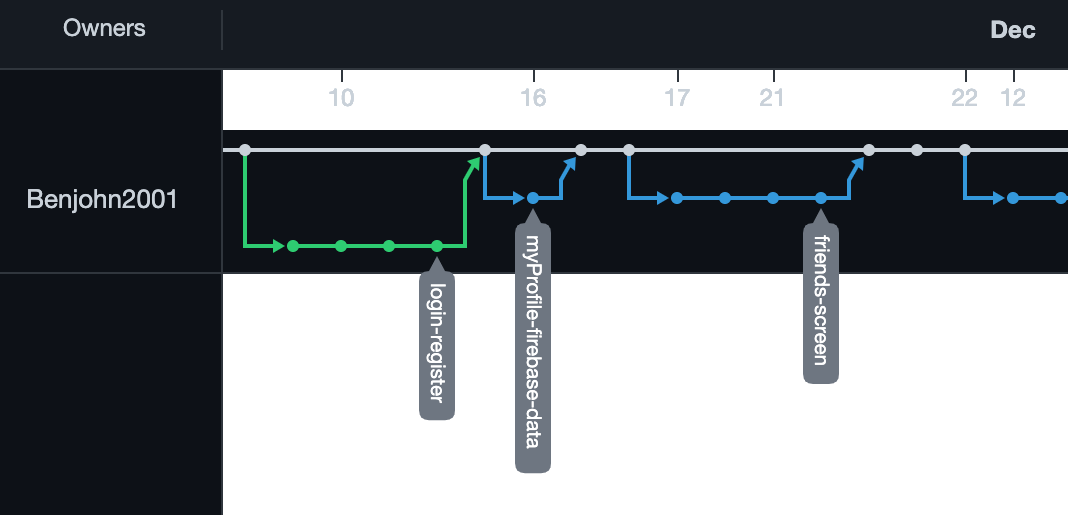
\includegraphics[width=\textwidth]{featureBranch.png}}
    \end{subfigure}
    \caption{Example of feature branching used in project}
    \label{fig:branching}
\end{figure}
\subsubsection{Issue Tracking}
The GitHub issue tracker was used to keep track of what tasks were still to be completed, along with any bugs that needed to be fixed. GitHub allows you to apply labels to an issue helping you to separate between Firebase and design issues for example (see \ref{fig:issues}).
\begin{figure}[!htbp]
    \centering
    \begin{subfigure}[b]{0.90\textwidth}
        \frame{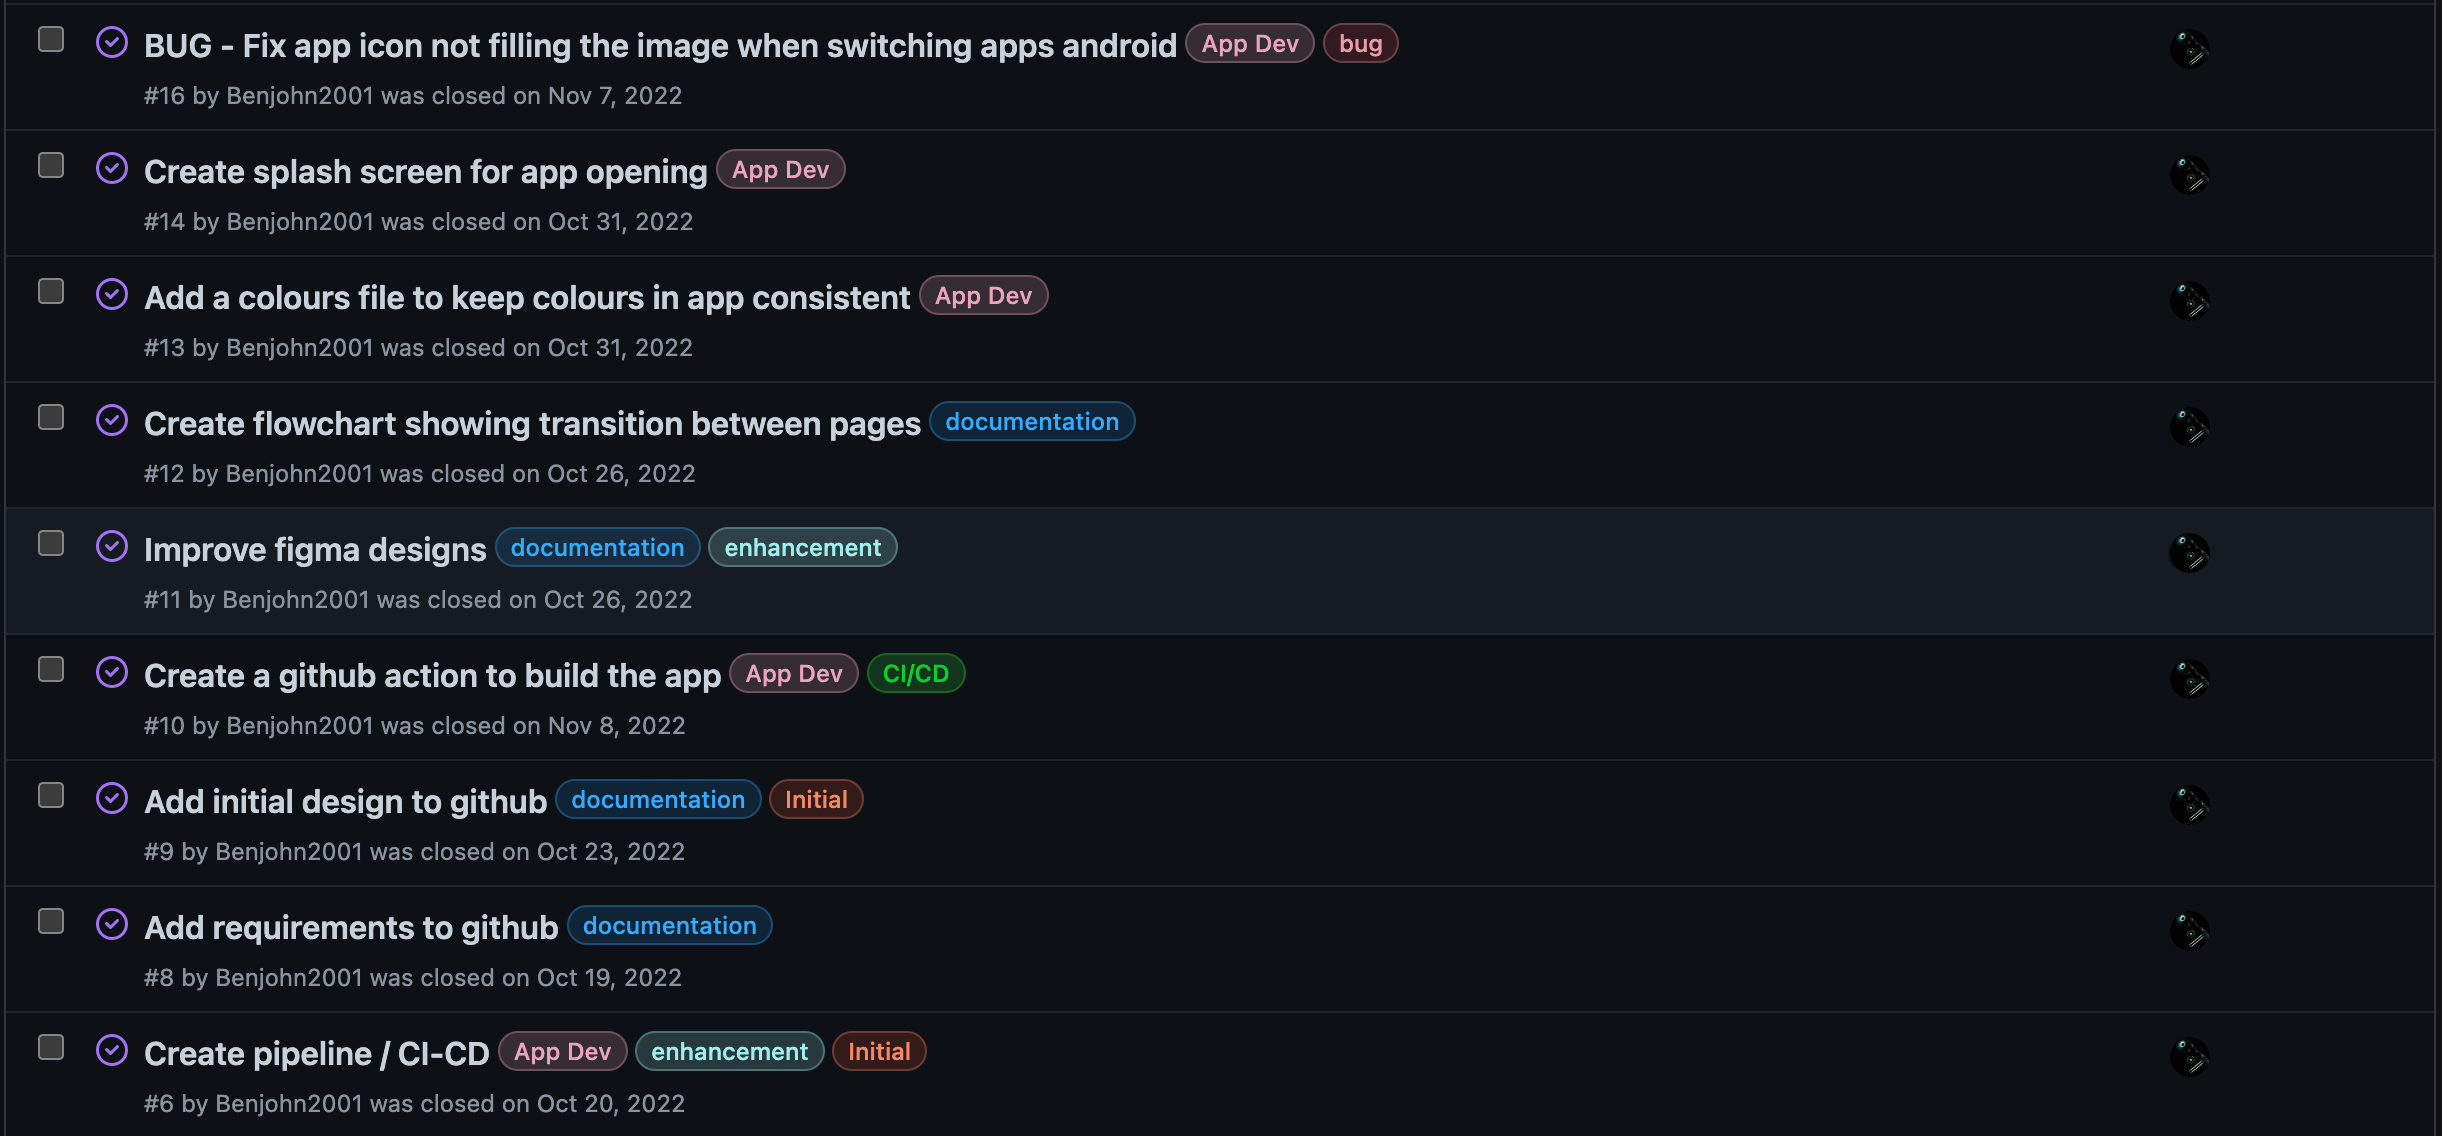
\includegraphics[width=\textwidth]{issues.png}}
    \end{subfigure}
    \caption{Examples of issues created in GitHub's issue tracker}
    \label{fig:issues}
\end{figure}
\subsubsection{Actions}
GitHub's actions is a continuous integration and continuous delivery tool that allows you to create workflows that are triggered on specific behaviour. A workflow that built and published the application upon a push to the main branch was created so that the newest version of the app was always accessible on my mobile device. A testing workflow was also created with any pushes to the tests, or main branch running the test suite along with code formatting and style checks (see \ref{CodeF&S}).
\section{Front End Technologies}
\subsection{React Native}
\subsubsection{Expo}
\subsubsection{JavaScript}
\subsection{Tailwind CSS}
\subsection{Code Formatting \& Style} \label{CodeF&S}
\subsubsection{ESLint}
\subsubsection{Prettier}

\section{Back End Technologies}
\subsection{Firebase}
\subsubsection{Authentication}
\subsubsection{Storage}
\subsubsection{Realtime Database}
